\documentclass[12pt,letterpaper]{article}
\usepackage{graphicx}
\usepackage{scrextend}
\usepackage{vmargin}
\usepackage{graphicx}
\usepackage{multirow}
\usepackage[utf8]{inputenc}
\usepackage[spanish]{babel}
\usepackage{multicol}
\usepackage{enumerate}
\usepackage{float}
\usepackage{amsmath, amsthm, amssymb, amsfonts}
\usepackage[usenames]{color}
\usepackage[breaklinks=true,hidelinks]{hyperref}
\spanishdecimal{.}
\parindent=0mm
\pagestyle{empty}
\definecolor{miorange}{rgb}{0.91, 0.43, 0.0}
\begin{document}
\setmargins{2.5cm}      
{1.5cm}                     
{2cm}  
{24cm}                    
{10pt}                          
{1cm}                          
{0pt}                             
{2cm}
\begin{titlepage}
\begin{center}

\includegraphics[scale=0.40]{../../../Logos/uanl.png} 
\hspace{2.5cm}

\includegraphics[scale=0.40]{../../../Logos/fcfm.png}
\end{center}
\vspace{2cm}
\begin{center}
\textbf{
UNIVERSIDAD AUTÓNOMA DE NUEVO LEÓN\\
FACULTAD DE CIENCIAS
FÍSICO MATEMÁTICAS}\\
\vspace*{2cm}
\begin{large}
\vspace{1cm}
\large{\textbf{Simuladores Moleculares}}\\
\textbf{Dinámica molecular con el potencial \\ de Lennard-Jones en dos dimensiones}\\
Omar Gonzalez Amezcua\\
\end{large}
\vspace{3.5cm}
\begin{minipage}{0.6\linewidth}
\vspace{0.5cm}
\changefontsizes{14pt}
Nombre:\\
Giovanni Gamaliel López Padilla\\
\end{minipage}
\begin{minipage}{0.2\linewidth}
\changefontsizes{14pt}
Matricula:\\
1837522
\end{minipage}
\end{center}
\vspace{4cm}
\begin{flushright}
\today
\end{flushright}
\end{titlepage}
\begin{multicols}{2}
\section*{Resumen}
\subsection*{Palabras clave}
\section*{Introducción}
\section*{Objetivo general}
\section*{Objetivo específico}
\section*{Marco teórico}
\begin{equation}
    \label{Potencial de Lennard-Jones}
    V(r) = 4 \epsilon \left[\left(\frac{\sigma}{r} \right)^{12} - \left(\frac{\sigma}{r} \right)^6 \right]
\end{equation}
donde:
\begin{itemize}
    \item $V$ es el potencial intermolecular entre dos átomos o partículas.
    \item $\epsilon$ es la profundidad del valle que define que tan fuerte es la atracción entre partículas.
    \item $\sigma$ es la distancia a la cual el potencial entre dos partículas es igual a cero.
    \item $r$ es la distancia de separación entre dos partículas
\end{itemize}
\begin{figure}[H]
    \centering
    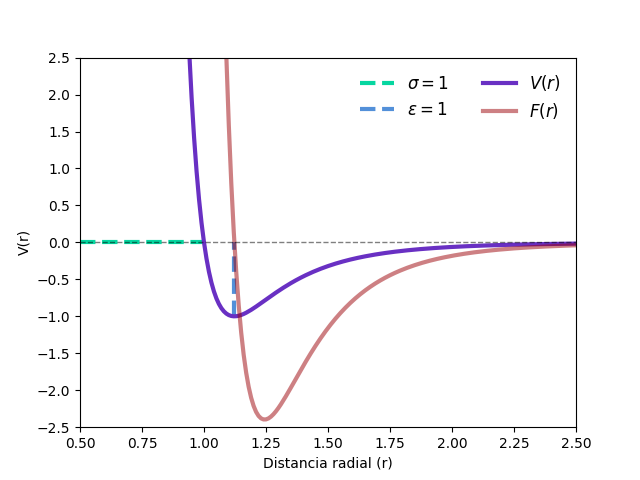
\includegraphics[scale=0.45]{../Graphics/Potencial.png}
    \caption{Potencial Lennard-Jones}
    \label{pot-len-jones}
\end{figure}
\section*{Resultados}
\begin{figure}[H]
    \centering
    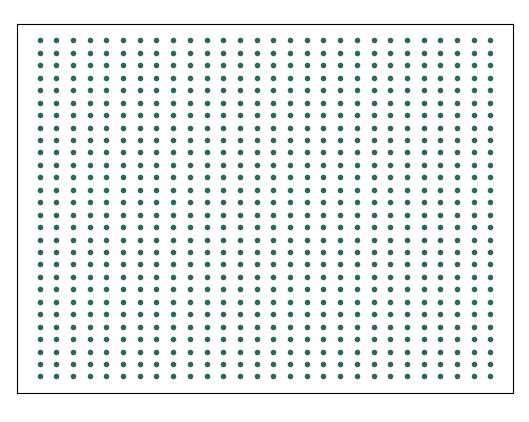
\includegraphics[scale=0.45]{../Graphics/Cor_in.png}
    \caption{Posición inicial de la dinámica}
    \label{pos inicial}
\end{figure}
\begin{figure}[H]
    \centering
    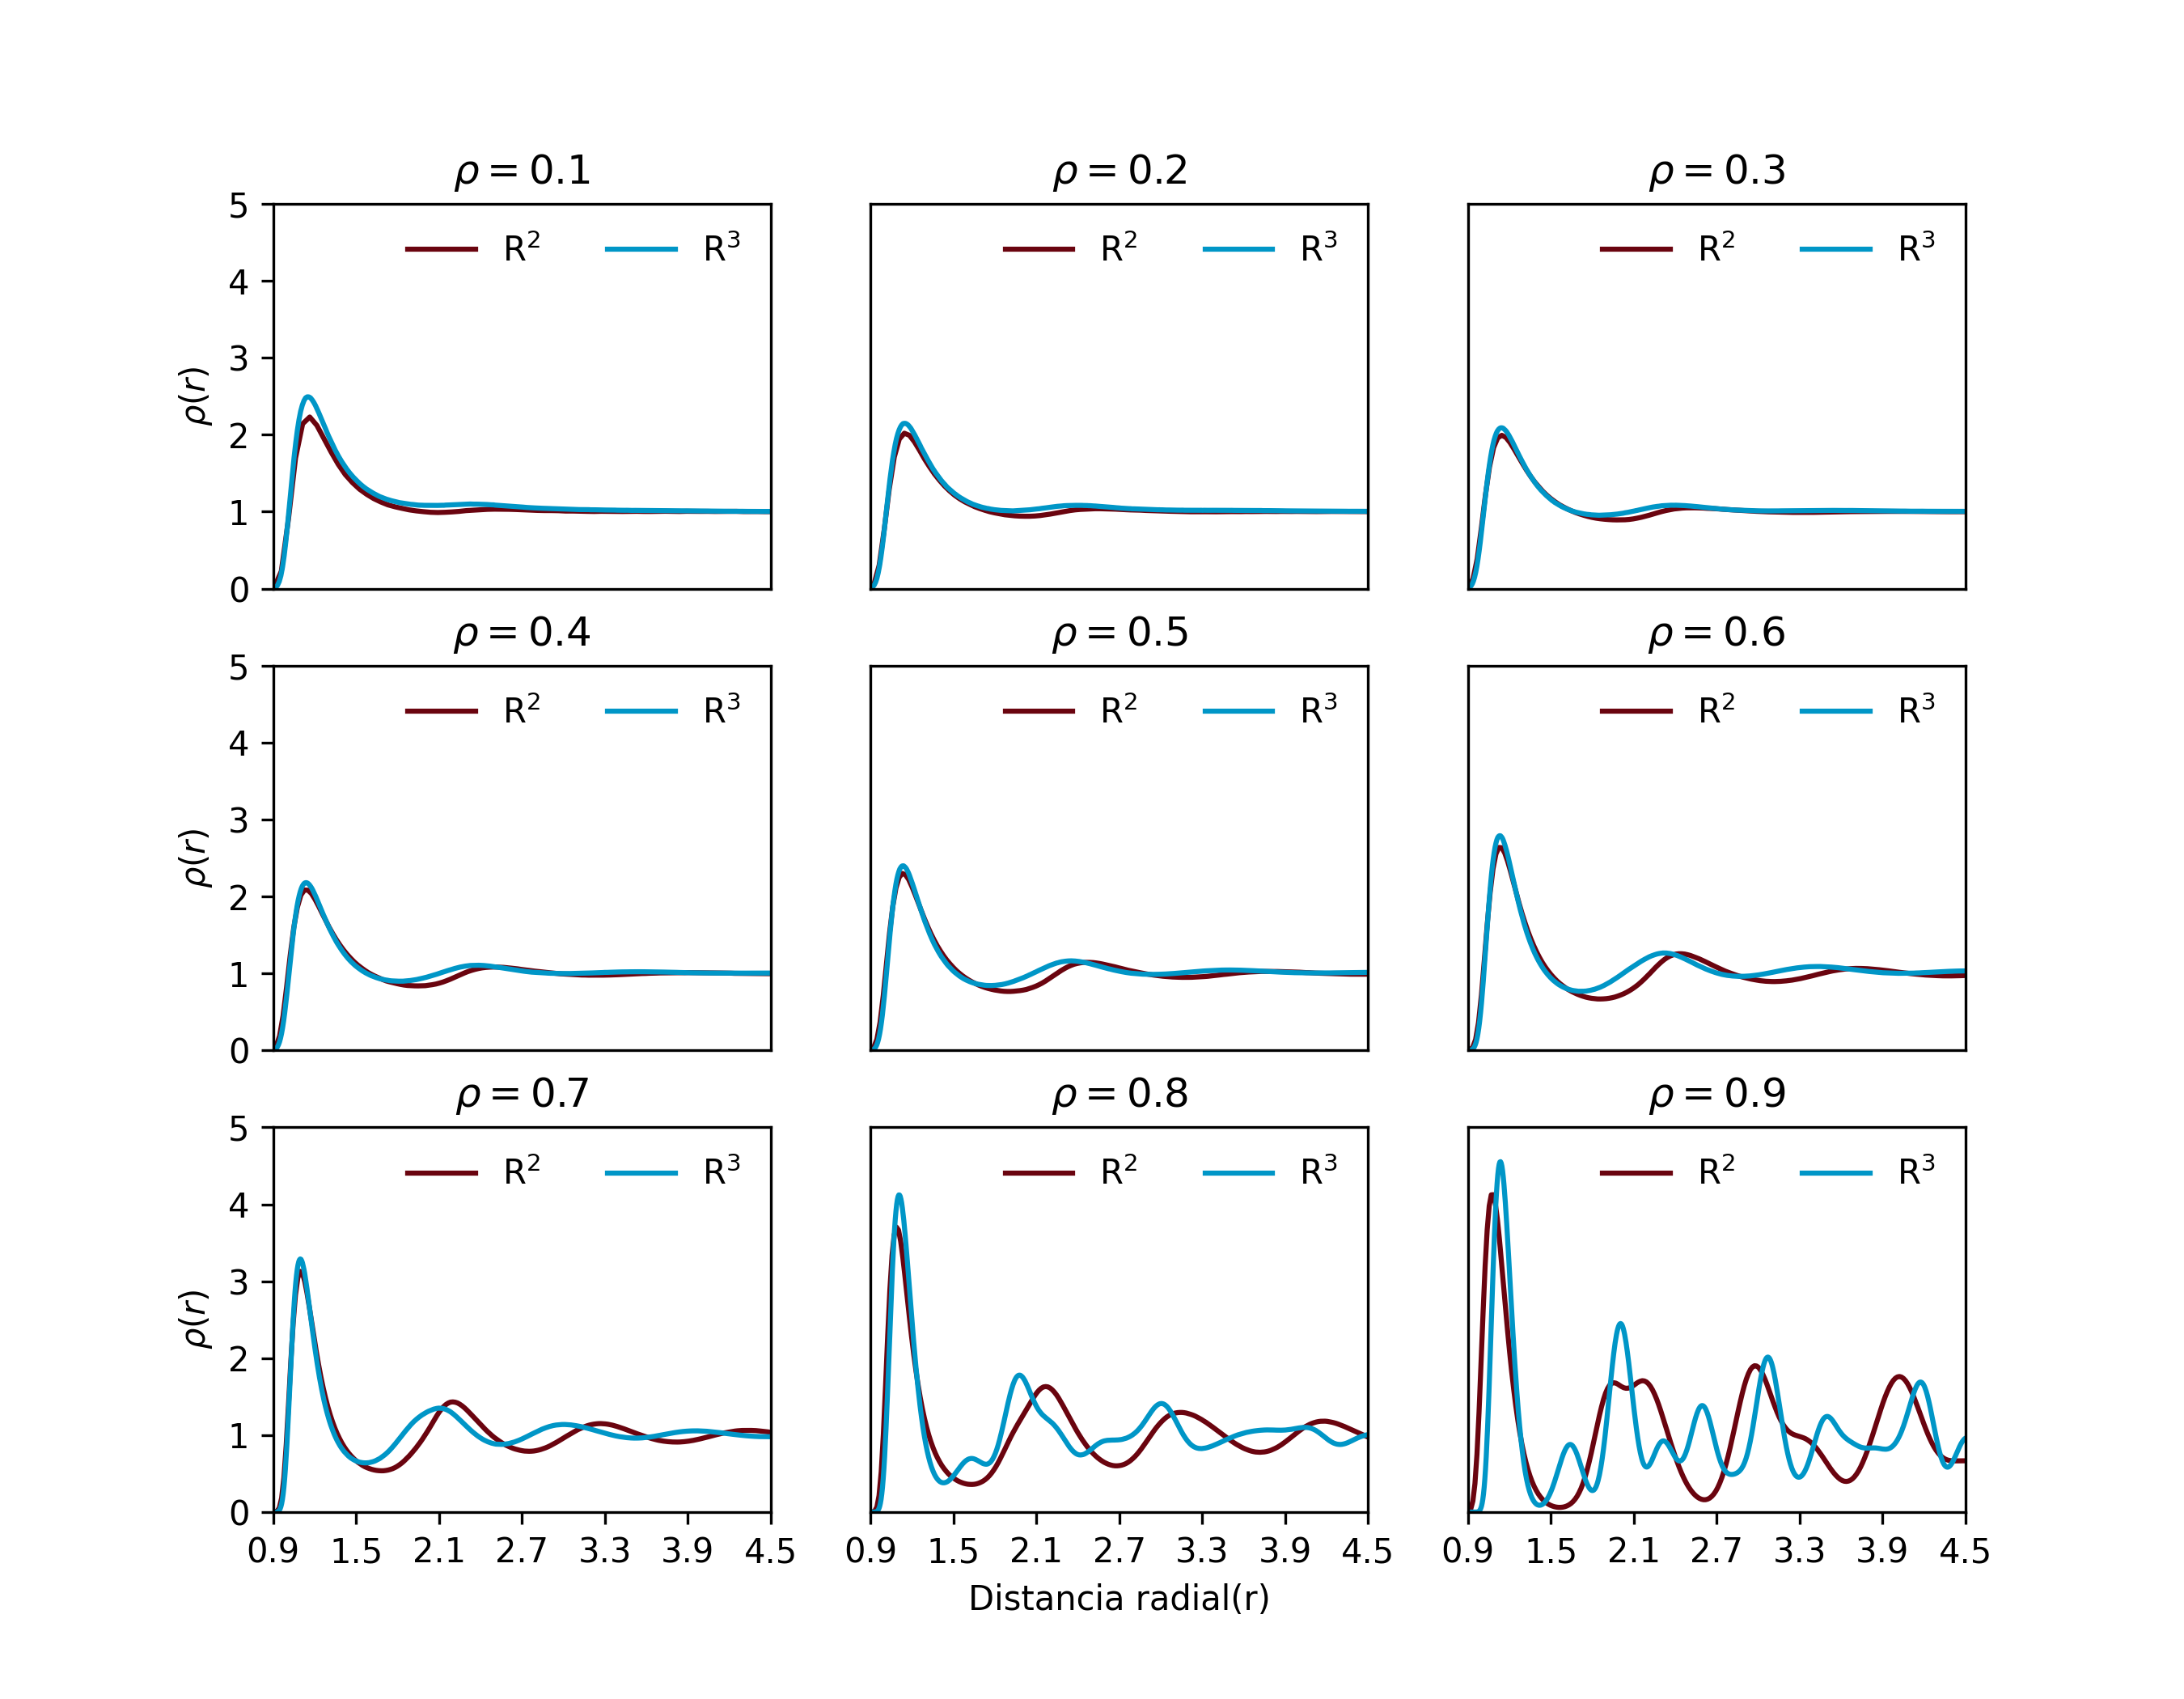
\includegraphics[scale=0.45]{../Graphics/Dis_rad.png}
    \caption{Distribución radial de la estructura}
    \label{distribucion radial}
\end{figure}
\begin{figure}[H]
    \centering
    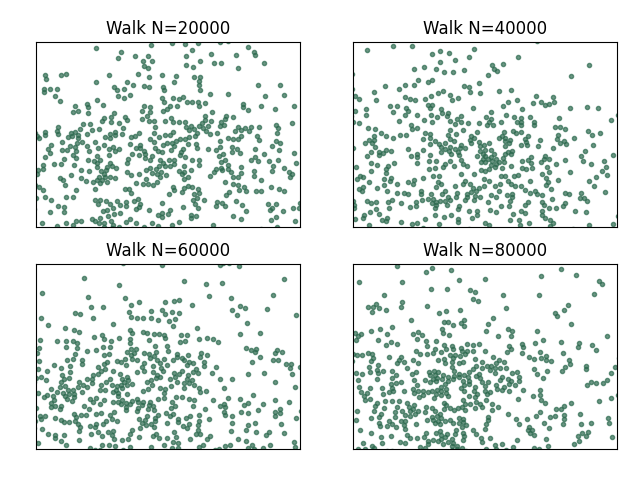
\includegraphics[scale=0.45]{../Graphics/Dim_Graphics.png}
    \caption{Dinámica molecular en diferentes tiempos}
    \label{screen dinamica}
\end{figure}
\begin{figure}[H]
    \centering
    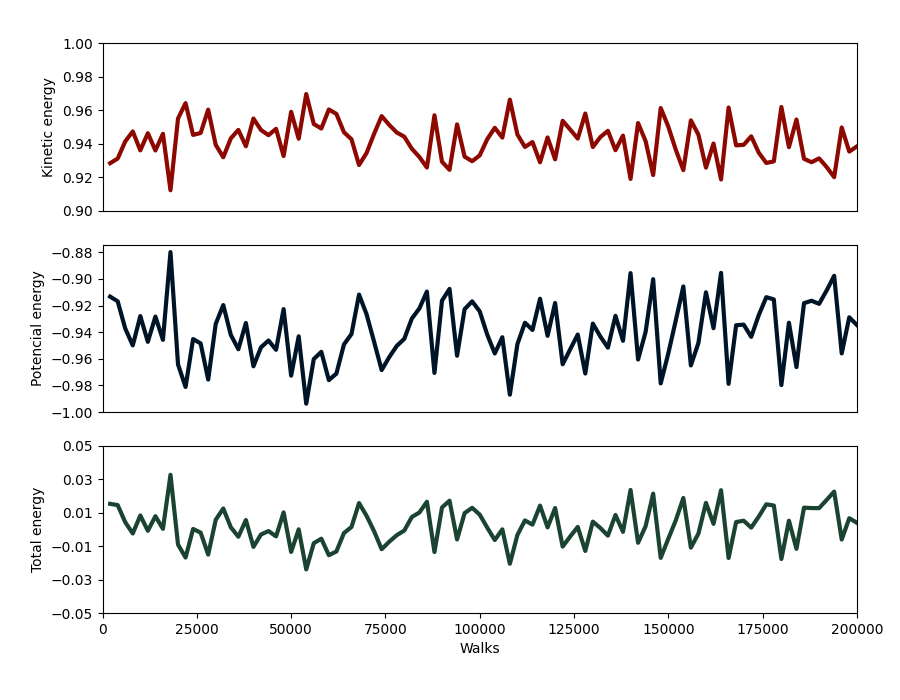
\includegraphics[scale=0.335]{../Graphics/Energy.png}
    \caption{Energía cinética, potencial y total del sistema en toda la simulación}
    \label{energias}
\end{figure}
\section*{Conclusiones}
\section*{Código}
\begin{itemize}
\item \href{https://github.com/giovannilopez9808/Notas_Agosto_2020/blob/master/Simulaciones/Proyecto_1/Scripts/MD-n3.f}{Github - MD-n3.f}\\
Este código contiene la simulación del sistema.
\item \href{https://github.com/giovannilopez9808/Notas_Agosto_2020/blob/master/Simulaciones/Proyecto_1/Scripts/Energy_Graphics.py}{Github - Gráfica de las energías}\\
Este código genera la gráfica \ref{energias}
\item \href{https://github.com/giovannilopez9808/Notas_Agosto_2020/blob/master/Simulaciones/Proyecto_1/Scripts/Cor_Graphics.py}{Github - Gráfica de la posición inicial y Distribución radial}\\
Este código genera la figura \ref{pos inicial} y \ref{distribucion radial}
\item \href{https://github.com/giovannilopez9808/Notas_Agosto_2020/blob/master/Simulaciones/Proyecto_1/Scripts/Dim_gif.py}{Github - Animación de la dinámica}\\
Este código genera la animación mostrada en la figura \ref{screen dinamica}
\item \href{https://github.com/giovannilopez9808/Notas_Agosto_2020/blob/master/Simulaciones/Proyecto_1/Scripts/Dim_Graphics.py}{Github - Gráfica para diferentes tiempos}\\
Este código genera la figura \ref{screen dinamica}

\item \href{https://github.com/giovannilopez9808/Notas_Agosto_2020/blob/master/Simulaciones/Proyecto_1/Scripts/Potencial_Graphics.py}{Github - Gráfica del potencial de Lennard-Jones}\\
Este código realiza la figura \ref{pot-len-jones}
\end{itemize}
\bibliographystyle{plain}
\bibliography{Main}
\nocite{*}
\end{multicols}
\end{document}